\documentclass{anvil-paper}
\usepackage{array}
\usepackage{float}
\newcommand{\Nm}{\mathrm{N\,m}}
\newcommand{\dd}{\,\mathrm{d}}
\title{Interface truncation and verified design gradients\\
in a nonlinear motor model}
\author{Robb Walters}
\date{October 2026}
\hypersetup{pdftitle={Interface truncation and verified design gradients in a nonlinear motor model},pdfauthor={Robb Walters},pdfsubject={Torque-ripple reproduction and discrete design-gradient verification}}

\begin{document}
\maketitle
\begin{abstract}
A motor optimization target can change with the numerical interface even
when average torque agrees closely. We reconstruct a published nonlinear
permanent-magnet motor with piecewise-linear finite elements and compare
conforming and harmonic rotor--stator coupling on identical meshes in our
GEODE implementation.
At the finest mesh, truncation at the reference's harmonic order 45 lowers
loaded torque standard deviation by 7--9\% and raises cogging standard
deviation by 59\%, relative to conforming coupling. Retaining every order
below the trace Nyquist limit reproduces conforming torque within a few
$10^{-9}$\,N\,m on the two checked meshes. Refining the independent reference
reduces its cogging discrepancy with GEODE from 12.9\% to 0.10\%, although neither sequence is fully converged.
For the saved optimized geometry, increasing interface order from 45 to 93
multiplies the aggregate squared ripple by 3.6 under fixed unscaled current,
while the initial objective rises only 16\%; the reduction remains above
2,400-fold across the tested models. We differentiate the converged nonlinear model through
mesh motion, excitation and torque evaluation. Among 704 distinct loaded
derivative comparisons, 688 agree with best-step central differences within
$2.8\times10^{-7}$ relatively; the largest error is $1.1\times10^{-5}$.
Ripple sensitivities nevertheless differ between the verified
model--estimator pairs. Fixing winding-group-1 density instead of current
reverses three mean-torque sensitivities at the initial design on the second-coarsest mesh, at order 45 and
full current.
The results separate discrete derivative accuracy from model-dependent
objectives and sensitivities; optimization time to a common validated
target remains to be measured.

\end{abstract}

\section{Introduction}
A small error in mean torque can conceal a large change in the quantity
being optimized. Reconstructing the initial motor of
\citet{wiesheu2024spline}, we find that truncating the interface at order 45
lowers loaded torque standard deviation by 7--9\% and raises cogging
standard deviation by 59\% on the finest mesh, relative to conforming coupling. The loaded
mean torque of either model agrees with the saved reference within 0.16\%.
Varying the transmitted order and checking the full-order identity
distinguish this model dependence from spatial refinement error. Rerunning
and refining the independent reference accounts for the initial cogging
discrepancy; checking the saved optimized geometry shows that interface
order also affects the reported design improvement.

The same distinction applies to derivatives. An adjoint can produce many
design sensitivities without a field solve per parameter
\citep{scotzniovsky2025}, but it differentiates the chosen discrete model
and excitation policy. It does not establish that the objective is
resolved, or that following its gradients beats a cheaper design model.
These questions require separate checks of the field model, derivatives
and optimization outcome.

We report a four-mesh comparison of conforming and truncated harmonic
coupling, including two torque estimators and a harmonic-order ladder.
We also verify derivatives of mean torque and ripple with respect to
12 design parameters at initial and perturbed designs, and expose the
effect of holding current rather than current density fixed. The
comparison shows how interface truncation and excitation policy affect
the objective and its sensitivities even when the discrete derivatives pass
verification. The numerical methods are established; the results supply
the evidence needed before comparing optimization costs.

\section{Related work}
\citet{wiesheu2024spline} combine spline-based rotor and stator shape
optimization with engineering parameters for a nonlinear permanent-magnet
synchronous motor. Their public implementation and saved outputs provide
the reproduction target here. Their related study combines parameter and
shape optimization with isogeometric analysis and compares against each alone
\citep{wiesheu2025combined}. We inherit the initial geometry, material
table and excitation conventions; we replace the field discretization and compare two
rotor--stator couplings. The resulting comparison is between numerical
models, rather than a comparison with a measured physical motor.

\citet{scotzniovsky2025} combine free-form deformation, differentiable
mesh warping and electromagnetic analysis with adjoint-based derivatives.
\citet{merkel2021shape} use isogeometric shape derivatives and harmonic
rotor--stator coupling to reduce electromotive-force harmonic distortion.
Their objective is electromotive-force distortion, and their validation
compares initial and optimized designs with a separate field solver.
Here we examine torque standard deviation in a nonlinear reconstruction
and test which interface model and excitation policy its gradients represent.

Harmonic weighting of a sliding interface was developed for finite-element
machine models by \citet{degersem2004harmonic}.
\citet{bontinck2018isogeometric} use separate isogeometric subdomains and
harmonic interface constraints; their exact circular geometry avoids
polygonal air-gap error. \citet{egger2022torque} derive torque from the
energy of a harmonic mortar formulation and examine its numerical
accuracy for ripple evaluation. Their linear-material cogging experiment
varies the maximum transmitted order from 39 to 129 and compares against
a refined order-200 reference. Thus torque sensitivity to interface order
is already established; our study quantifies its effect on loaded nonlinear
ripple, a saved optimized design, and design sensitivities.
Bontinck et al. also analyze stability as the multiplier space grows
relative to the field space, so adding orders requires compatible spatial
resolution. We compare coupling torque with the
gap-averaged stress expression of \citet{arkkio1987}. These works motivate
checking interface order, field resolution and torque evaluation together,
rather than treating small mean-torque error as sufficient validation.
The sensitivity of cogging-torque prediction to finite-element
discretization and evaluation method was examined by \citet{howe1992cogging};
\citet{arkkio2012proper} study mesh selection for torque computation.

\citet{ion2018robust} compare deterministic gradient-based optimization
with stochastic search for electric devices, including a permanent-magnet
motor, using geometry parametrizations that avoid remeshing. Extending
that comparison here requires competitive inexpensive models and evaluation
of all candidates against a common refined target.

\citet{kemmetmueller2015} use nonlinear magnetic equivalent circuits for
torque control, including saturation and nonsinusoidal behavior. Their
control problem differs from shape optimization, but it demonstrates why
saturation alone does not establish the need for a full-field model.
\citet{roomi2022} develop a waveform-targeting surrogate for electrical
machine design, while \citet{wen2023} adapt reduced models along a
shape-optimization trajectory in fluid examples. These approaches motivate
waveform-aware and adaptive baselines. Their published performance is not
transferred to the motor studied here.

\section{Motor model and reconstruction}
\subsection{Geometry and operating states}
The full machine has six poles and 36 stator slots. We model a
$60^\circ$ sector, occupying $60^\circ\leq\theta\leq120^\circ$ at zero
rotation, with antiperiodic conditions on the radial boundaries. The rotor
inner and outer radii are 16 and 44\,mm; the stator inner and outer radii
are 45 and 67.5\,mm. Axial length is $L=0.1$\,m. The 1\,mm air gap is
split at the coupling radius $r_c=44.5$\,mm. Figure~\ref{fig:geometry}
shows the material-tagged reconstruction.

\begin{figure}[htbp]
\centering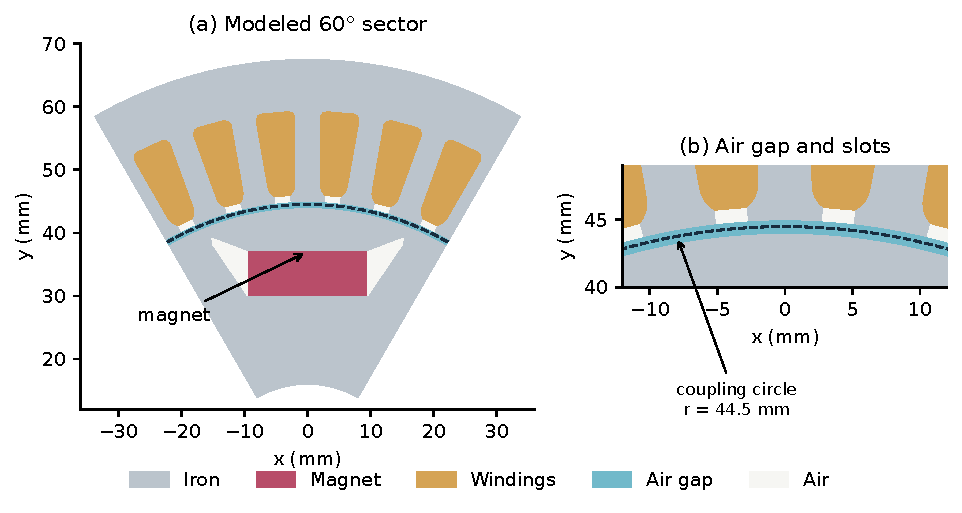
\includegraphics[width=\linewidth]{figures/geometry.pdf}
\caption{Initial-design geometry rendered directly from the committed
coarsest mesh. The dashed line is the rotor--stator coupling circle. The
right panel enlarges the gap and slot openings. Material boundaries are
shown without the element edges; the geometry is not an optimized result.}
\label{fig:geometry}
\end{figure}

The reconstruction uses the initial NURBS exports in the public snapshot.
Their control points are stored with weights already multiplied in, and
patch orientation must be accounted for when integrating areas. Two thin
rotor patches described as air slits in source comments receive iron under
the reference's material assignment; we follow that assignment. The
mesh generator preserves the winding groups separately, since their two
characteristic areas are approximately 36.29 and 31.22\,mm$^2$.

At mechanical angle $\beta$, phase currents are
\begin{equation}
 I_q(\beta)=a I_*\sin(\phi_0+3\beta+\delta_q),\qquad
 (\delta_U,\delta_V,\delta_W)=(0,-2\pi/3,2\pi/3),
 \label{eq:current}
\end{equation}
where $a\in\{0,0.5,1\}$, $I_*=9.677657374$\,A, and the electrical phase
offset $\phi_0=0$ for the initial design. Angles in
Eq.~\eqref{eq:current} are in radians. Each winding group carries current
density $J_g=12s_g I_q/|\Omega_g|$, with its own area and prescribed sign
$s_g\in\{-1,1\}$. Using a common area would change the current density
between groups by about 16\%. We compare 20 distinct mechanical angles,
$0^\circ,1^\circ,\ldots,19^\circ$, excluding the duplicated endpoint in
the source CSV. The reference's optimization grid contains the ten even
angles; both grids are retained in the artifacts.

\subsection{Nonlinear field equation}
The two-dimensional magnetic vector potential $A=A_z$ determines the
flux density $\mathbf B=(\partial_y A,-\partial_x A)$. Iron is described
by an isotropic reluctivity $\nu(|\mathbf B|^2)$, where reluctivity is
the inverse of permeability. For a test function $v$ that satisfies the
homogeneous constraints, the weak equation is
\begin{equation}
 \int_\Omega \nu(|\nabla A|^2)\nabla A\cdot\nabla v\dd\Omega
 =\int_\Omega J_z v\dd\Omega
  +\int_{\Omega_m}\mathbf M\cdot(\partial_y v,-\partial_x v)\dd\Omega.
 \label{eq:weak}
\end{equation}
Here $\mathbf M$ denotes the permanent-magnet source in
$\mathbf H=\nu\mathbf B-\mathbf M$. In the magnet,
$\mu_r=1.05$ and $B_r=1.4$\,T, so its source magnitude is
$H_c=B_r/(\mu_0\mu_r)$, not $B_r/\mu_0$. Its direction is $\pi/2$
in the rotor frame and rotates with the rotor. Air and windings have
$\mu_r=1$. The inner and outer circular boundaries have $A=0$.

We use continuous piecewise-linear triangles. With nodal vector $u$,
element gradients $g_i=\nabla\varphi_i$, $G=\nabla A$ and $s=G\cdot G$,
the residual derivative on one element is
\begin{equation}
 K^e_{ij}=|\Omega_e|\left[\nu(s)g_i\cdot g_j
       +2\nu'(s)(g_i\cdot G)(g_j\cdot G)\right].
 \label{eq:tangent}
\end{equation}
The second term is required when the material changes with field strength.
Newton steps use this consistent tangent, with damping and a stopping
reference independent of the initial guess. Constant potential offsets,
where allowed by the boundary conditions, do not change that reference.
The solver reports whether it stopped at the requested tolerance or an
estimated floating-point floor. All 500 baseline and sensitivity solves, and all 1,140
additional harmonic-coupling solves, stopped at the requested tolerance.

The iron law uses 47 tabulated M27 $B$--$H$ points from 0 to 2.30\,T.
Monotonicity is imposed on $H(B)$, not on $\nu(B^2)=H(B)/B$.
The tabulated $H/B$ is non-monotone up to about 0.75\,T.
The two material tangent eigenvalues must satisfy
\begin{equation}
 \nu>0,\qquad \nu+2s\nu'=\frac{\dd H}{\dd B}>0.
\end{equation}
The GEODE and reference interpolants agree to round-off between 0.05 and
2.25\,T. GEODE uses an odd cubic near zero and a continuous slope into the
vacuum-slope tail above 2.30\,T. The reference uses a low-field clamp and
a different last-knot slope. The maximum relative difference in
reluctivity near zero is 6.66\%; the last segment differs in $H$ by at
most $2.17\times10^{-4}$ relatively. We test the torque effect of the
low-field difference in Section~\ref{sec:sensitivity}.

\subsection{Rotation and torque}
At the modeled angles, the two circular traces have matching nodes after
rotation. Our conforming interface identifies their potentials, including
the antiperiodic sign on sector wrap-around. Writing the full nodal vector
as $u=P\hat u+u_D$, the reduced residual and tangent are
$\hat R=P^T R(P\hat u+u_D)$ and $\hat K=P^T K P$.
The rotor geometry and magnet source rotate together; currents use the
same mechanical angle in Eq.~\eqref{eq:current}.

We average Maxwell stress over the air gap using the Arkkio expression
\citep{arkkio1987}
\begin{equation}
 T(\beta)=\frac{L}{\mu_0(r_2-r_1)}
  \int_{\Omega_{\rm gap}}r B_r B_\theta\dd\Omega,
 \qquad(r_1,r_2)=(44,45)\ {\rm mm}.
 \label{eq:torque}
\end{equation}
Positive torque acts counter-clockwise on the rotor. All torques in this
paper include axial length and refer to the modeled sector. We apply no
factor of six when comparing with the saved reference arrays, despite a
per-length label appearing in the reference evaluation plots.

The alternative harmonic model imposes
\begin{equation}
 \int_{\Gamma_c}(A_s-A_r)e_n\dd\Gamma=0,\qquad
 e_n\in\{\sin(n\theta),\cos(n\theta)\},\quad n=3,9,\ldots,45.
\end{equation}
The 16 constraints match the reference's eight orders. Rotor and stator
retain distinct trace unknowns. With constraint matrix $C$, Lagrange
multipliers $\eta$ and reduced potential $\hat u$, Newton's method uses
the saddle tangent
\begin{equation}
 \begin{bmatrix}K&C\\ C^T&0\end{bmatrix}.
\end{equation}
The trace moments use the exact Fourier integrals of the piecewise-linear
hats. Rotation enters their centers; the constrained energy derivative gives
\begin{equation}
 T_c=-L\eta^T\frac{\partial(C^T\hat u)}{\partial\beta},
 \label{eq:couplingtorque}
\end{equation}
with the state held fixed in the partial derivative, consistent with
\citet{egger2022torque}. Forward comparisons use Arkkio for both GEODE
couplings to isolate the interface change; coupling torque is a separate
check. The derivative study uses coupling torque for the harmonic model
and Arkkio for the conforming model. The two objectives and their gradients
are consequently comparisons of those specified model--estimator pairs.

The main harmonic runs retain antiperiodic trace-end pairing. An additional
set frees those ends, matching the reference's treatment. Increasing the
transmitted orders to every mode below the trace Nyquist limit reproduces
the conforming Arkkio torques within $4.1\times10^{-9}$\,N\,m on L0 and
$1.3\times10^{-9}$\,N\,m on L1. This checks the interface implementation
without fitting any parameter to the saved torque.

\section{Verification and experiment design}
The nonlinear implementation is checked against linear assembly, residual
finite differences, a manufactured solution and a saturated annulus with
an independent radial field relation. Solver verification records are
linked in the data-availability section; motor derivative checks appear
in Section~\ref{sec:gradients}.

Sector tests compare the constrained solution with a full-machine solve,
check the reduced tangent by finite differences, and exercise positive,
negative and wrapped rotation steps. Clockwise and counter-clockwise
triangle orderings give equivalent magnet sources and fields. The motor
regression also detects changes in magnet strength, magnet direction,
phase ordering and rotation direction.

The motor study uses four meshes, L0--L3, with 3,153, 9,937, 36,083 and
139,268 nodes. The $60^\circ$ coupling arc has $120\cdot2^\ell$ segments at level
$\ell$, so integer-degree rotation is represented at every level.
Each level contains 60 baseline solves: three current levels and 20
angles. A solution at one angle initializes the next angle at the same
current. We report the mean and population standard deviation,
\begin{equation}
 \bar T=\frac1N\sum_{k=1}^N T_k,\qquad
 \sigma_T=\left[\frac1N\sum_{k=1}^N(T_k-\bar T)^2\right]^{1/2},
 \quad N=20.
\end{equation}
The standard deviation is the ripple metric used for the comparison.
At zero current it measures cogging, the torque variation caused by the
permanent magnets and slots without applied phase current.

For a scalar statistic $q$, the estimated L3 refinement interval is
\begin{equation}
 q_3\ \pm\ e_q,\qquad
 e_q=\max\{|q_2-q_1|,|q_3-q_2|\}.
 \label{eq:band}
\end{equation}
We use the same construction pointwise for waveforms. This interval is a
refinement diagnostic, not a proven error bound or a statistical confidence
interval. It does not cover reference-model error or angular quadrature
error. The loaded means change direction between the last two increments,
so a last-increment estimate alone would be particularly weak.

\section{Forward reproduction results}
\subsection{Coupling changes the ripple objective}
Table~\ref{tab:torque} compares the same geometry, material and excitation
with two interface models. The conforming L3 means are 0.15\% and 0.16\%
low at half and full current. Harmonic coupling reduces the mean deviations
to $-0.002\%$ and $+0.051\%$, with both reference means inside the estimated
refinement intervals. The loaded ripple deviations fall from $+9.9\%$
and $+11.3\%$ to $+1.7\%$ and $+1.3\%$.

\begin{table}[htbp]\centering\small
\caption{L3 population standard deviation and mean torque, in N\,m per
sector, on the 20-angle grid. The last column gives ripple deviation from the
saved reference; n/a identifies the reference itself. The reference is
subsequently refined in Section~\ref{sec:refinement}.}
\label{tab:torque}
\begin{tabular}{llrrr}\toprule
Current fraction & Model & Mean & Std & Std vs ref. (\%)\\\midrule
0 & Reference & 0.00010 & 0.01071 & n/a \\
0 & Conforming & 0.00001 & 0.00760 & -29.1 \\
0 & Harmonic & 0.00000 & 0.01209 & +12.9 \\
0.5 & Reference & 0.66208 & 0.03895 & n/a \\
0.5 & Conforming & 0.66106 & 0.04279 & +9.9 \\
0.5 & Harmonic & 0.66206 & 0.03961 & +1.7 \\
1 & Reference & 1.44248 & 0.07935 & n/a \\
1 & Conforming & 1.44023 & 0.08829 & +11.3 \\
1 & Harmonic & 1.44322 & 0.08036 & +1.3 \\
\bottomrule\end{tabular}

\end{table}

Figure~\ref{fig:waveforms} shows the improvement angle by angle. The largest
full-current difference falls from 0.0272 to 0.0034\,N\,m. The harmonic
full-current ripple interval contains the saved reference; the saved half-current
value lies approximately $5\times10^{-5}$\,N\,m below its interval.
Mean agreement is therefore insufficient to characterize waveform accuracy.

\begin{figure}[!t]\centering
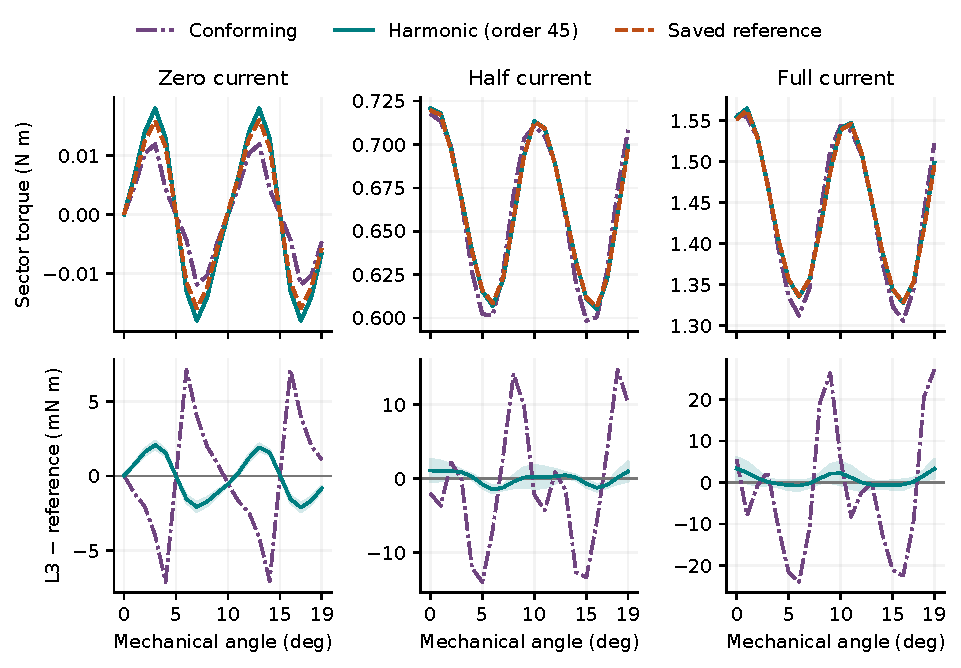
\includegraphics[width=\linewidth]{figures/coupling-waveforms.pdf}
\caption{Top: L3 torque for conforming and order-45 harmonic coupling,
compared with the saved reference. Bottom: each GEODE waveform minus the
reference; shading is the harmonic model's pointwise estimated refinement
interval from Eq.~\eqref{eq:band}. Residual panels have independent scales.
All GEODE curves use Arkkio torque, so the paired difference changes the
coupling while holding the estimator fixed. The saved reference is coarse;
Section~\ref{sec:refinement} reports its refinement.}
\label{fig:waveforms}\end{figure}

The saved zero-current reference exposes a separate discretization effect. Harmonic coupling changes the
cogging standard deviation from 29.1\% below to 12.9\% above the reference.
Its waveform is close to a 1.13-fold scaling of the saved waveform, but the
reference lies outside the estimated ripple interval. This motivates
refining the reference itself before interpreting the discrepancy. The harmonic cogging standard deviations are
0.0101, 0.0119, 0.0121 and 0.0121\,N\,m on L0--L3, compared with
0.0107\,N\,m in the reference. The independent reference refinement below tests this coarse-model
explanation directly.

\subsection{Spatial resolution and transmitted order}
Spatial refinement at fixed order and order refinement on a fixed mesh
answer different questions (Fig.~\ref{fig:convergence}). At L3, order 45
raises cogging standard deviation by about 59\% and lowers loaded
standard deviation by 7--9\%, relative to the conforming values. At L1 and L2,
order 189 approaches the conforming torque to within $1.1\times10^{-4}$\,N\,m.
A spatially refined order-45 solution thus remains a solution of a
truncated interface model. Matching that truncation improves reproduction
of the published calculation; it does not establish which model better
represents the physical motor.

\begin{figure}[!t]\centering
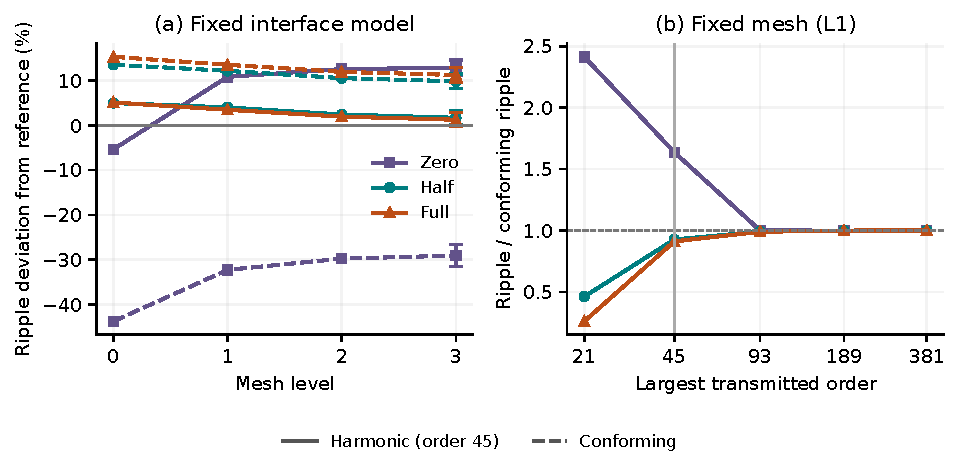
\includegraphics[width=\linewidth]{figures/coupling-convergence.pdf}
\caption{Left: ripple deviation from the reference under spatial
refinement, with solid lines for harmonic order 45 and dashed lines for
conforming coupling; L3 bars use Eq.~\eqref{eq:band}. Right: order
refinement on L1 with logarithmic order spacing, normalized by the
conforming ripple at that same level.
The saved reference uses order 45; see Section~\ref{sec:refinement} for its
refinement. Colors identify current, not coupling.}
\label{fig:convergence}\end{figure}

Two additional controls narrow the explanation. At L3, coupling torque
and the inner- and outer-half Arkkio estimates are each within
$9\times10^{-5}$\,N\,m of full-band Arkkio in the order-45 solution.
Freeing the coupling-arc ends changes torque by less than
$5.4\times10^{-5}$\,N\,m. These effects are too small to explain the remaining
cogging gap at the tested resolution.

\subsection{Sensitivity controls}\label{sec:sensitivity}
The controlled changes in Table~\ref{tab:sensitivity} are too small to
explain the observed waveform gap at the tested settings. The near-zero
material difference has particularly little effect on torque despite its
6.66\% local reluctivity difference. This is a measured sensitivity of
the initial design and does not establish insensitivity after optimization.

\begin{table}[htbp]\centering\small
\caption{Maximum absolute torque change relative to the baseline at the
same mesh level, using conforming coupling and Arkkio torque. Entries
summarize the recorded angle/current subsets.}
\label{tab:sensitivity}
\begin{tabular}{p{.48\linewidth}ll}\toprule
Change & Levels & Max. $|\Delta T|$ (N\,m)\\\midrule
Reference low-field interpolation and clamp & L2, L3 & $2.1\times10^{-6}$\\
Relative Newton tolerance $10^{-12}$ vs $10^{-8}$ & L2; L3 full current & $7.3\times10^{-8}$\\
Exact winding areas vs mesh areas & L2 & $3.9\times10^{-4}$\\
Inner or outer half of the Arkkio band & L3 & $7.3\times10^{-5}$\\
\bottomrule\end{tabular}
\end{table}

In the recorded estimator study, single-circle Maxwell-stress estimates
vary more with the integration radius than the half-band Arkkio estimates.
The paired coupling-torque and half-band checks above avoid selecting a
favorable radius. A post-processing filter of the solved conforming field
also gives non-monotone ripple changes across the tested cuts and currents;
it does not replace a field solve with a truncated interface. The complete
filter results are retained in the accompanying forward-study records.

\subsection{Independent reference refinement}\label{sec:refinement}
We rerun the public reference with its own degree-two isogeometric model,
harmonic orders $3,9,\ldots,45$ and coupling torque, at $3$, $6$, $12$ and
$24$ subdivisions in each patch direction. The $3\times3$ rerun first
reproduces all 60 saved torques with differences at most $9.8\times10^{-13}$\,N\,m.
The run uses Octave 11.3.0, GeoPDEs revision \texttt{53ae5ca1} and nurbs
1.4.3; compatibility edits, source hashes and raw records are retained.
The corresponding field degrees of freedom are 4,079, 12,518, 43,220
and 159,920.

The reference cogging standard deviation changes from 0.01071 to 0.01220,
0.01212 and 0.01208\,N\,m (Fig.~\ref{fig:validation}a). GEODE L3 at order
45 gives 0.01209\,N\,m, a 0.10\% difference from the finest reference.
The maximum pointwise discrepancy drops from $2.1\times10^{-3}$ to
$3.4\times10^{-5}$\,N\,m. At half and full current, the finest reference
standard deviations are 0.03947 and 0.08014\,N\,m; GEODE is 0.35\% and
0.27\% higher (panel b). All five finest-reference statistics, the three
standard deviations and two loaded means, lie within GEODE's L3
refinement intervals. The coarse saved reference therefore accounts for
the cogging mismatch in Section 5.1 at the matched interface order.

This agreement still concerns finite discretizations. The last cogging
increments approximately halve; extending that trend would put a limit
near 0.0120\,N\,m, an estimate without a bound. The last two half-current
standard-deviation increments are both about $-0.3\%$ and do not shrink;
we therefore leave its remaining error unestimated. The 0.10\% cogging
agreement is a comparison of finite-resolution values, not an accuracy
bound; neither refinement sequence is fully converged.
Tightening the reference Newton stopping threshold from $10^{-6}$ to
$10^{-14}$ changes the checked cogging torques by at most
$4.4\times10^{-8}$\,N\,m. GEODE retains straight-sided geometry, and the
high-field extrapolation of the iron law has not been varied in a paired
torque experiment. Neither cross-code agreement nor refinement proves
physical accuracy for the machine.

\subsection{Validation of the saved optimized design}\label{sec:opt120}
The saved reference design at iteration 120, denoted Opt120, includes
12 scalar parameters and ten grouped surface-control offsets. We evaluate
its full exported geometry on freshly generated meshes; simply moving
the finest initial mesh produces four inverted triangles. Its inner
air-gap band no longer has the annular area assumed by the full-band
Arkkio functional, so harmonic results here use coupling torque.
Conforming results use only outer-band Arkkio on the fresh exported mesh.
On the same L3, order-45 Opt120 field at full current, the outer-band and
coupling estimates differ by about $1.3\times10^{-4}$\,N\,m in mean and
$1.1\times10^{-5}$\,N\,m in standard deviation. This paired check supports
the estimator substitution at this resolution.
This estimator restriction is specific to these geometries; it does not
validate outer-band Arkkio on arbitrary moved meshes or stator offsets.

Define $F=\sum_{a\in\{0,0.5,1\}}\sigma_T(a)^2$, in
$\mathrm{N^2\,m^2}$, on the 20-angle grid. With the evaluation current
held fixed in the unscaled geometry, raising the transmitted order from
45 to 93 multiplies Opt120's $F$ by 3.6, from $1.07\times10^{-6}$ to
$3.86\times10^{-6}$ (Fig.~\ref{fig:validation}c). The initial design's
$F$ rises by 16\%. Its ratio to Opt120 is consequently 7,631 at order 45,
2,454 at order 93 and 2,444 for conforming coupling. The full-current
Opt120 standard deviation rises from 0.00066 to 0.00164\,N\,m.
The large ripple reduction survives these checks, but its magnitude
depends strongly on the interface model. Between L2 and L3, changes in
$F$, normalized by L3, reach 1.36\% for the initial design and 2.71\%
for Opt120 across the three models; these increments are not error bounds.
For Opt120 at order 45, the successive L1--L2 and L2--L3 increases in $F$
are $3.05\times10^{-8}$ and $2.90\times10^{-8}$\,N$^2$\,m$^2$,
so they barely shrink and do not establish an asymptotic rate. An alternate
freshly constructed mesh family changes by 3.22\% from L2 to L3.
The $2.79\times10^{-6}$\,N$^2$\,m$^2$ interface effect is about
96 times the last export-mesh increment, despite this unresolved remainder.
A possible explanation is that optimization against order 45 favors
cancellation within that truncated model. This is a conjecture, not an
ablation result: increasing the order raises full-current ripple but
lowers Opt120 cogging standard deviation from 0.00061 to 0.00035\,N\,m.

Current policy also changes feasibility (panel d). At L3 and order 45,
the initial full-current mean is 1.4433\,N\,m. Opt120 gives 1.3147\,N\,m
under fixed \emph{unscaled} current, 1.2550\,N\,m under fixed physical
current, and 1.4983\,N\,m under the reference's fixed group-1 density rule.
The first two are 8.9\% and 13.0\% below the initial mean; the density-rule
value is 3.8\% above it. These policy comparisons use the same Opt120
geometry, but comparisons with the initial motor also change size:
Opt120 shortens the stack from 100 to 80\,mm and has radial scale
$s=1.0477$, unscaled outer diameter 130.293\,mm and operating angle
$-11.646^\circ$ (Table~\ref{tab:parameters}). Every Opt120 torque carries
the explicit size factor $s^2L/(0.1\,\mathrm{m})=0.878175$.
Removing both size factors from the fixed-unscaled-current mean gives
1.4971\,N\,m, 3.7\% above the initial mean; normalizing only length to
100\,mm while retaining the actual radial scale gives 1.6434\,N\,m.
These algebraic normalizations separate the size factors from the current
rule; they are not reoptimized designs. Opt120 is outside the prospective
fixed-size, fixed-physical-current problem.

A separate reproduction comparison uses the saved reference current at
each design, rather than fixed unscaled current. At Opt120, GEODE's
order-45 full-current mean is 1.4986\,N\,m versus 1.5000\,N\,m in the
saved arrays, but its standard deviation is $3.53\times10^{-4}$ versus
$1.76\times10^{-4}$\,N\,m, a factor of 2.0. The half-current values are
$5.53\times10^{-4}$ and $4.37\times10^{-4}$\,N\,m.
The largest pointwise difference across the two loaded currents is about
$2.1\times10^{-3}$\,N\,m. With this matched current policy and zero-current
values included, the initial-to-Opt120 objective ratios are 10,170 for
GEODE and 11,982 for the saved reference. The 7,631 ratio above instead
holds unscaled current fixed. Reference refinement was run only at the
initial design, so the cause of the Opt120 discrepancy remains unresolved.

Angular sampling becomes more consequential at this low ripple. Relative
to the 40-angle grid, the ten-angle Opt120 objective reads about 1.05\%
high at order 45 and 5.90\% low at order 93 on the fresh L3 mesh; the
conforming value reads 17.1\% low. The accompanying records retain shifted
20-angle grids and withheld currents 0.25 and 0.75. Candidate validation
must check these effects at the candidate, since initial-design agreement
alone would miss them. All 3,240 solve rows in the 18 successful records used for
these candidate comparisons stopped at tolerance.

\begin{figure}[!t]\centering
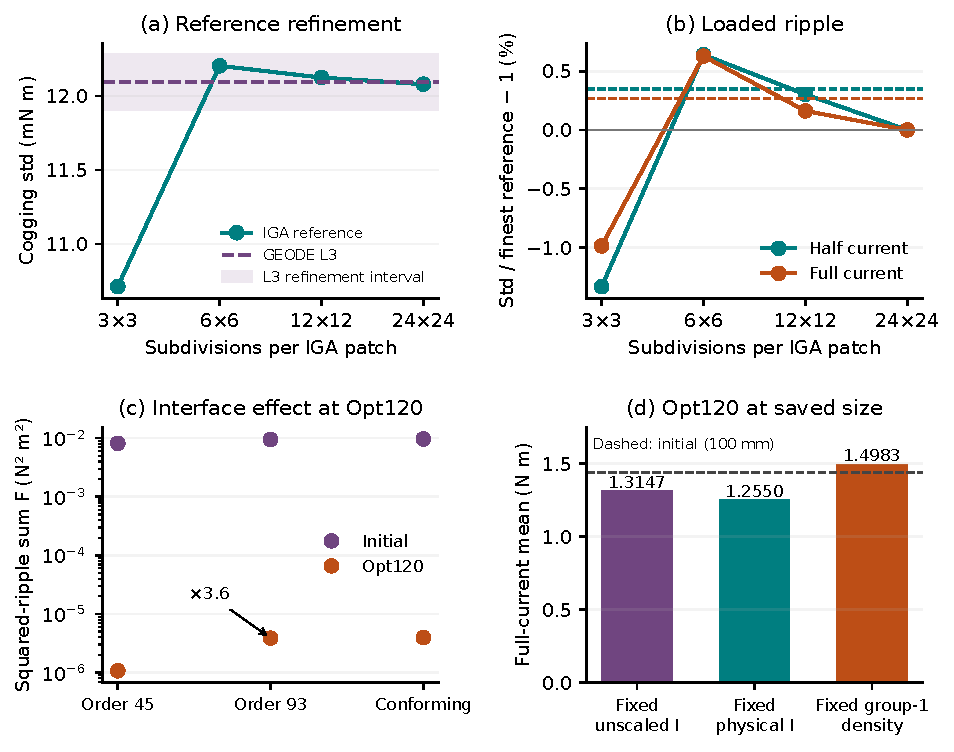
\includegraphics[width=\linewidth]{figures/refined-validation.pdf}
\caption{Reference and candidate validation from raw torque records.
(a) Independent IGA reference cogging refinement at order 45; the dashed
line is GEODE L3 and its shaded band uses Eq.~\eqref{eq:band}.
(b) Loaded standard deviation relative to the finest
reference at each current; circles are IGA, horizontal lines are GEODE L3.
The finest IGA point is zero by construction.
Panels (a,b) use the initial geometry and 20 angles; GEODE uses Arkkio,
with coupling torque checked separately. (c) Initial and Opt120 squared
ripple sums at L3 on fresh meshes and 20 angles, under fixed unscaled
current. Harmonic values use coupling torque; conforming values use
outer-band Arkkio. (d) Full-current mean at order 45 for Opt120 under
three current rules at its saved size; the dashed line is the initial
mean at the initial size. All candidate
values use coupling torque.}\label{fig:validation}
\end{figure}

\section{Design-gradient verification}\label{sec:gradients}
\subsection{Differentiated model and excitation policy}
For a design vector $p$, the converged state $z$ contains the reduced
potential and, for harmonic coupling, its multipliers. Writing the full
constrained residual as $R(z,p)=0$, the discrete adjoint is
\begin{equation}
 R_z^T\psi=F_z^T,\qquad
 \frac{\dd F}{\dd p}=F_p-\psi^T R_p.
 \label{eq:adjoint}
\end{equation}
We differentiate mesh coordinates, element terms, magnet sources, current
loads, harmonic constraints and the torque functional. The explicit
coordinate derivative of Arkkio is included for conforming coupling.
Fixed-topology mesh motion $X(p)$ supplies the chain rule
$\dd F/\dd p_k=\langle\dd F/\dd X,\partial X/\partial p_k\rangle$
for geometric parameters, with direct terms added where needed.

The 12 parameters comprise nine geometric lengths (MAG, MH, MW,
SW1--SW4, SD1 and Sr1), axial length, operating angle and radial scale.
The two designs are the initial parameters and an interior point halfway
toward the saved optimized scalar parameters
(Appendix~\ref{sec:parameters}). This verifies a local scalar
parametrization. The reference's optimized geometry also uses grouped
surface-control displacements; reproducing its 12 scalar values alone
does not reproduce that geometry. The present gradient comparison does
not include derivatives of those additional groups or a new optimized
motor.

In this scalar derivative study, fixed current means fixed peak current
in the unscaled geometry, so
$J_g=12s_g I_q/|\Omega_g(X)|$ changes when a slot changes area.
For comparison we implement the reference optimizer's rule, denoted
\emph{fixed group-1 density}: $I_*\propto |\Omega_1(X)|s$, where $s$ is
radial scale, with the proportionality constant fixed at the initial
design. The unscaled geometry is evaluated and torque is multiplied by
$s^2$, following the reference. Both rules agree at the initial geometry
but have different derivatives. Group-2 density is not held fixed because
the ratio of the two winding areas can change. At L1 (harmonic coupling,
coupling torque, full current), the mean-torque derivative with respect to SW1 is
$+1.68$\,N\,m/m under fixed current and $-220.85$\,N\,m/m under fixed
group-1 density (Fig.~\ref{fig:gradients}). SW1 is the stator-tooth-width
parameter. The sign change comes from the additional winding-area/current
term: a wider tooth narrows the slot and lowers current under fixed
group-1 density. At this state the policy changes seven of the ten
geometric/scale derivatives and reverses the mean-torque signs for SW1,
SW4 and SD1. Rotor parameters MAG, MH and MW leave winding area unchanged
and therefore give identical derivatives under the two rules. The prospective
fixed-size problem sets radial scale to one, making fixed physical and
unscaled current coincide. A future
optimization comparison must hold this policy fixed across methods.

\subsection{Finite differences and Taylor remainders}
The derivative objectives are mean torque and population standard
deviation on the ten even mechanical angles, matching the reference's
optimization grid. Central differences move the same mesh at $p\pm h e_k$;
step sweeps separate truncation from floating-point and nonlinear-solve
error. We also check the first-order remainder
$|F(p+h e_k)-F(p)-h\,\dd F/\dd p_k|$ for quadratic decay.

Across initial and perturbed designs, L0--L2 and the recorded loaded
current/rule subsets, there are 800 objective--parameter records. They pool
harmonic/coupling-torque and conforming/Arkkio evaluations. The fixed-density
MAG, MH and MW records repeat 96 fixed-current comparisons byte-for-byte,
leaving 704 distinct comparisons. Of these, 688 have a best-step relative
error at most $2.8\times10^{-7}$; the maximum is $1.07\times10^{-5}$ for
a small Sr1 ripple derivative. This is a best-step verification statistic,
not the accuracy of a finite-difference step chosen in advance.
Figure~\ref{fig:gradients} includes the 704 distinct cases and an explicit
Taylor sweep. The artifact retains every step, rejected displacement and
relative error. The recorded subsets do not form a full factorial study.

\begin{figure}[!t]\centering
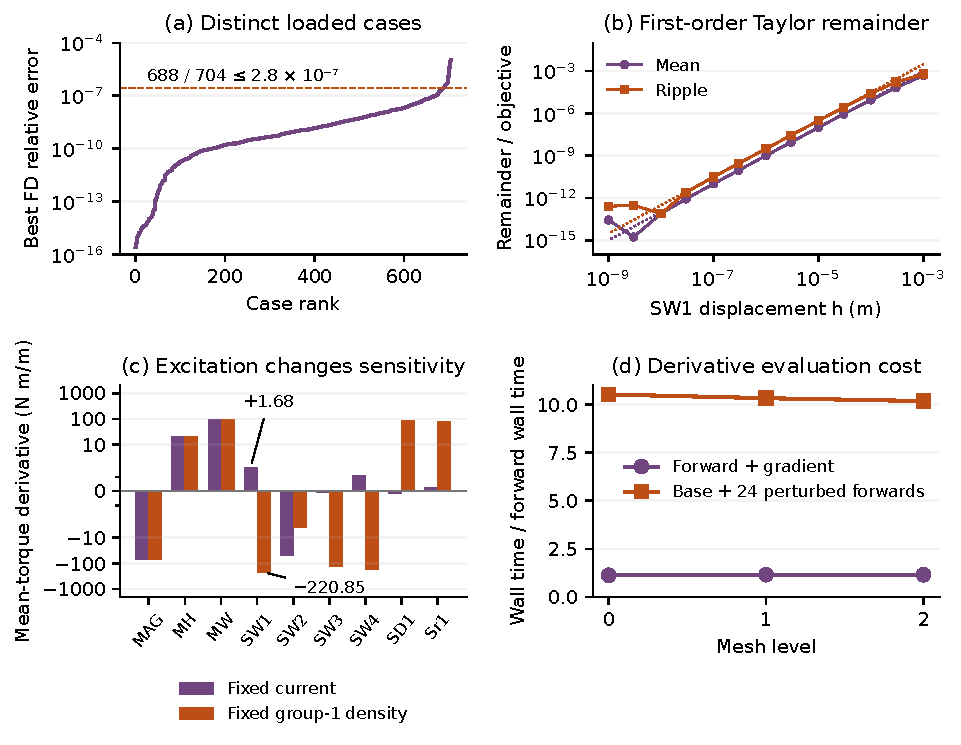
\includegraphics[width=\linewidth]{figures/design-gradients.pdf}
\caption{Discrete gradient evidence. (a) The 704 distinct loaded best-step
finite-difference errors, sorted, pooling harmonic/coupling-torque and
conforming/Arkkio objective--parameter cases. (b) SW1 Taylor remainders at L1, initial design,
full current, harmonic coupling and coupling torque, fixed current; the
plotted remainders are divided by $|F(p)|$, and dotted $h^2$ guides are anchored at $h=10^{-5}$\,m. (c) Mean-torque sensitivities for the nine geometric
parameters under two current rules at that same state; the vertical axis
is symmetric-log, linear within $\pm2$\,N\,m/m. (d) Recorded cost
ratios for harmonic coupling at tolerance $10^{-14}$; gradients include
the forward evaluation, and FD includes its shared base forward.
L0/L1 use medians of three runs, L2 a single run.
These timing data were collected under uncontrolled host load.}
\label{fig:gradients}\end{figure}

After removing duplicates and the analytic axial-length and radial-scale
cases, 530 of 592 loaded comparisons have an anchored quadratic-remainder
window spanning at least four decades in step size; 388 span at least five.
The window is the contiguous run where remainder/$h^2$ stays within a
factor of two of its value at $h=10^{-5}$\,m (or $10^{-2}$ degrees for
operating angle). Smaller gradients reach round-off sooner. An anchored-window diagnostic fails for the initial-design, full-current
conforming/fixed-density SW1 ripple cases at L0 and L1 because the remainder changes sign near the anchor; their
widest quadratic windows span two decades. The nearly cancelling
zero-current mean is a weaker check: its best relative errors reach
$7.0\times10^{-4}$. Cogging standard-deviation errors are at most
$8.9\times10^{-7}$. Thus the loaded agreement does not describe every
zero-current derivative.

Discrete derivative accuracy also does not imply mesh convergence. In the
harmonic model, SW3 mean-torque sensitivities change sign between coarse
levels and their increments shrink with refinement; ripple gradients converge
more slowly than most mean gradients. The conforming/Arkkio SW2 mean
sensitivity is non-monotone across L0--L3 ($-46.5$, $-41.3$, $-44.4$,
$-47.2$\,N\,m/m), whereas harmonic/coupling torque approaches $-47.1$
from $-49.8$\,N\,m/m. Fresh-remesh checks of MW, SW1 and SW2 are limited
at small steps by changes in connectivity. The L2 MW mean-derivative fit
has relative gap $2.6\times10^{-6}$, but individual remeshed steps at
$h\geq10^{-4}$\,m scatter by about $6\times10^{-4}$. The largest L2 full-current
remeshed-versus-moved fitted discrepancy is 3.8\% for the SW1 ripple
derivative. These checks support the discrete chain rule while leaving
refinement of candidate designs necessary.

\subsection{Model dependence of verified sensitivities}
The two model--estimator pairs give different ripple sensitivities even
at the same design (Fig.~\ref{fig:modelgradients}). At L2 and full fixed
current, the MAG ripple derivative is 1.28\,N\,m/m for harmonic/coupling
torque versus 1.94 for conforming/Arkkio at the initial design. At the
perturbed design the values are 0.75 and 1.87\,N\,m/m. These differences
persist under mesh refinement. At L3 the MAG pairs are 1.22 versus 1.87
at the initial design and 0.57 versus 1.67\,N\,m/m at the perturbed design.
In particular, the latter harmonic component changes appreciably even
though the vector norm changes by about 1\%. Mean-torque
sensitivities agree more closely in the box-scaled comparison: the
Euclidean norm of the vector difference, divided by the conforming vector
norm, is 0.58\% and 0.66\% for the mean at the initial and perturbed
designs, versus 6.7\% and 10.2\% for ripple. The norm weights the largest
components most heavily: the initial SW2 and SW3 mean components differ
by 6.5\% and 17\% relative to conforming values.
At L3, the ripple gaps remain 6.58\% and 10.25\%, while each model
changes by 0.46--1.19\% from L2 to L3. The mean gaps fall to 0.16\%
and 0.26\%; the conforming model itself changes by 0.52--0.54\%.
The L2 mean gap is therefore comparable to spatial refinement, whereas
the ripple gap persists beyond the measured refinement increments. Because the
estimator changes with the model, this experiment measures their combined
effect; it does not isolate an interface-only derivative error or establish
which gradient is closer to the physical machine.

\begin{figure}[!t]\centering
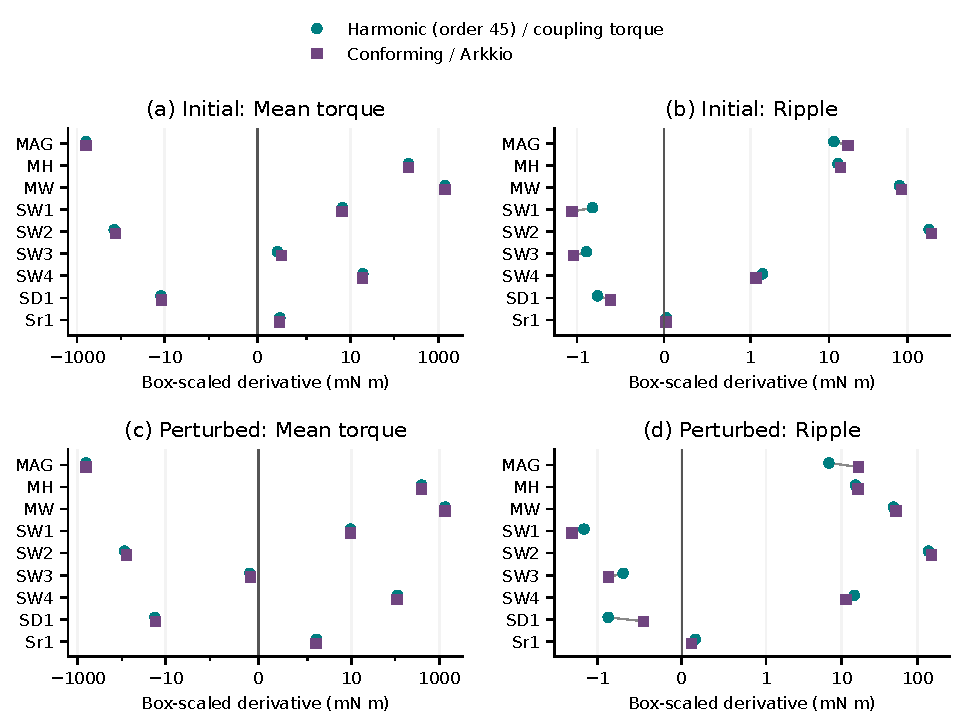
\includegraphics[width=\linewidth]{figures/model-gradients.pdf}
\caption{Full fixed-current sensitivities at L2, scaled by each geometric
parameter's reference box width $w_k$. Top: initial design; bottom:
perturbed design. L3 MAG values and refinement changes are given in the
text. Left: mean torque; right: standard deviation. The plotted
quantity $w_k\partial q/\partial p_k$ is a local sensitivity, not a finite
change across the box. Coupling and torque estimator both differ between
the two series. Gray segments join the two estimates for each parameter. Horizontal axes are symmetric-log, linear within
$\pm1$\,mN\,m. All nine widths, in mm, are 9, 10, 15, 4, 3, 1, 18, 70 and
1.5 in the displayed order.}\label{fig:modelgradients}
\end{figure}

\subsection{Recorded derivative cost}
The recorded timings use an Apple M3 Ultra with 28 cores, default solver
threading, and concurrent host load averaging 14--24. The effective thread
count was not pinned. A forward evaluation covers ten angles, starts from
zero, and warm-starts successive angles. The full gradient includes that
forward, ten torque adjoints, mesh derivatives and contractions for all
12 parameters and both aggregate objectives. Both aggregates reuse the
per-angle torque derivatives. Central differences use 24 forward sweeps,
each warm-started from the base states, at step $h=10^{-6}$ in each
parameter's stored unit (m, degrees or dimensionless scale). We add the
shared base forward to the recorded 24-sweep FD time for a common starting
point. These derivative timings are a separate workload from the 1,640
forward validation solves.

Across L0--L2, both couplings and tolerances $10^{-8}$ and $10^{-14}$, the
full gradient costs 1.13--1.20 forwards, whereas central differences cost
8.2--10.5 including the shared base solve. Table~\ref{tab:cost} gives the harmonic tight-tolerance subset.
Shape-map setup is recorded separately and must be included in a complete
optimization budget. The cost ratio concerns derivative evaluation
on one loaded host. It provides no measurement of optimizer iterations,
surrogate calibration cost or time to a validated target.

\begin{table}[H]\centering\small
\caption{Recorded harmonic-model cost at relative tolerance $10^{-14}$,
initial design and full current. Times are seconds for ten-angle sweeps;
FD includes the shared base sweep, and setup is a one-time shape-map cost.}
\label{tab:cost}\begin{tabular}{lrrrr}\toprule
Mesh & Forward & Forward + gradient & Base + FD & Setup\\\midrule
L0 & 0.664 & 0.748 & 6.997 & 0.011 \\
L1 & 3.174 & 3.658 & 32.811 & 0.041 \\
L2 & 12.702 & 14.644 & 129.390 & 0.222 \\
\bottomrule\end{tabular}

\end{table}

\section{Discussion and limitations}
The controlled interface change explains most of the loaded ripple gap
while preserving mean-torque agreement. The order ladder shows why this
matters for optimization: interface truncation changes the objective even
as spatial error decreases. The paired gradient comparison also measures
changes in ripple sensitivities despite small discrete derivative errors.
The saved optimized design retains a large ripple reduction after the
checks reported here, while its objective increases 3.6-fold with
interface order and its mean-torque comparison depends on both motor size and current policy.

The model is two-dimensional and magnetostatic. It does not evaluate
thermal behavior, demagnetization, fatigue, end effects, losses or a
complete efficiency map. The comparison uses published computational
artifacts, with no new measurements on a physical motor. The forward comparisons cover the initial and saved optimized designs;
local derivative tests at an interior scalar design do not validate an
entire optimization trajectory. The reference refinement is at the initial
design. Denser and shifted angle grids and additional currents are checked
for Opt120, but new candidates require their own refinement.

The prospective optimization comparison fixes outer diameter (SD1), axial length,
radial scale, operating angle and physical peak current, and compares eight
geometric scalars with those scalars plus ten grouped offsets. Exact-gradient,
derivative-free and empirical radial-basis-surrogate methods will be assessed
against predeclared 50\%, 90\% and 99\% ripple-reduction targets, using a
common order-93, L2, 20-angle validation with numerical and mean-torque
margins and final L3, 40-angle checks. All costs count toward a budget of
60 measured validation-forward wall times; unattained targets remain
censored. There are no matched optimization results in this paper, and
an empirical surrogate alone cannot establish an advantage over a reduced
physical model.

A cheap waveform or reduced physical model is an essential baseline.
The linear slotless screening control in Appendix~\ref{sec:slotless}
admits a three-coefficient angular fit at one geometry. That does not
establish generalization across shapes, but it cautions against inferring
an optimization advantage from parameter count or adjoint cost alone.

\section{Conclusion}
On identical meshes of a published nonlinear motor, order-45 truncation
lowers loaded torque standard deviation by 7--9\% and raises cogging
standard deviation by 59\% relative to conforming coupling at L3.
Refining the independent reference reduces the initial cogging discrepancy
from 12.9\% to 0.10\% at matched order, although neither sequence is fully
converged and the remaining error is not bounded. For the saved optimized
design, raising the interface order from 45 to 93 multiplies the
squared-ripple objective by 3.6 while preserving a reduction above
2,400-fold. Its shorter stack and changed radial scale must be separated
from current policy when comparing mean torque with the initial motor;
at its saved size it exceeds the initial mean only under the density rule
among the three policies tested.
Design gradients pass finite-difference and Taylor checks at two parameter
points, while the cross-model ripple-sensitivity gap persists under
refinement. The excitation rule reverses three mean sensitivities at the
initial L1, order-45, full-current state. Derivative verification therefore
does not settle objective resolution or feasibility. A practical speedup
still requires optimization against inexpensive baselines at a common
independently refined target.

\section*{Code and data availability}
The original forward and gradient evidence is fixed at GEODE commit
\href{https://github.com/rjwalters/geode-fem/tree/910593bad6f64f9f01671c2632b57034e72b9c61}{\texttt{910593ba}}.
The repository contains the
\href{https://github.com/rjwalters/geode-fem/tree/910593bad6f64f9f01671c2632b57034e72b9c61/benchmarks/motor_reference/forward_harmonic}{raw motor runs and analysis},
\href{https://github.com/rjwalters/geode-fem/tree/910593bad6f64f9f01671c2632b57034e72b9c61/benchmarks/motor_reference/geometry}{geometry and mesh-generation scripts},
\href{https://github.com/rjwalters/geode-fem/tree/910593bad6f64f9f01671c2632b57034e72b9c61/benchmarks/motor_shape_gradient/design}{design-gradient sweeps and timing records},
and \href{https://github.com/rjwalters/geode-fem/tree/910593bad6f64f9f01671c2632b57034e72b9c61/benchmarks/motor_nonlinear_m1}{solver verification logs}.
Candidate-validation records are pinned at
\href{https://github.com/rjwalters/geode-fem/tree/224332c526be1191183af82b610973c7778de720/benchmarks/motor_validation}{\texttt{224332c5}},
and independent reference reruns at
\href{https://github.com/rjwalters/geode-fem/tree/8acd21ecf85d89fe077275a3c04ca70b53963d43/benchmarks/motor_reference/reference_refinement}{\texttt{8acd21ec}}.
Reference data are extracted from the authors'
\href{https://github.com/MichaelWiesheu/ICEMsnapshot/tree/b145aaf4ab1a6424828bc941eaf172f48fa0d458}{ICEM snapshot at \texttt{b145aaf4}},
a later repository revision rather than a claim to the original conference
release. Source hashes, extraction checks and the upstream GPL-3.0-or-later license
are retained. The paper package includes a manifest, copied figure inputs
and a regeneration script; it does not require rerunning FEM to rebuild
the figures. Recomputing the physical study requires the separately
documented mesh and solver commands; the benchmark READMEs record the
GEODE-side Gmsh and Rust toolchain versions.

\appendix
\section{Linear slotless screening control}\label{sec:slotless}
The stored slotless model has 24 distinct angles. Fitting
$T(\phi)=c_0+c_1\cos\phi+c_2\sin\phi$, with electrical angle $\phi=p\theta_r$, mechanical rotor angle $\theta_r$
and pole-pair count $p$, on alternate angles and
evaluating on the other twelve gives normalized held-out RMSE
$3.08\times10^{-10}$ and maximum error $6.82\times10^{-10}$, using the
recorded analytic-amplitude normalization. This is a locked-rotor angle sweep,
not synchronous operating ripple. For a fixed linear field operator and
sinusoidal sources, the field lies in a small basis of source responses;
a quadratic torque functional can contain only the corresponding finite
set of harmonics. The particular model needs just the three fitted
coefficients. This is an angular interpolation test at one geometry,
not a shape-gradient test or evidence of generalization across designs.

\section{Design points for derivative checks}\label{sec:parameters}
Table~\ref{tab:parameters} identifies the scalar derivative-study coordinates
and the saved Opt120 coordinates. Values are rounded for display; the accompanying records
retain full precision. The operating angle is stored in degrees and
converted to radians in the current equation. These coordinates describe
the scalar design space; the saved reference optimum additionally contains
surface-control offsets.
\begin{table}[H]\centering\small
\caption{Initial and interior perturbed design points for derivative
checks, alongside Opt120 for the forward validation. Lengths refer to the
unscaled geometry; surface-control offsets are retained in the data.}\label{tab:parameters}
\begin{tabular}{l>{\raggedright\arraybackslash}p{.28\linewidth}lrrr}\toprule
Parameter & Meaning & Unit & Initial & Perturbed & Opt120\\\midrule
MAG & Pole-axis iron depth above magnet & mm & 7.0000 & 6.5506 & 6.1011 \\
MH & Radial magnet height & mm & 7.0000 & 4.8722 & 2.7444 \\
MW & Magnet width & mm & 19.0000 & 19.8670 & 20.7340 \\
SW1 & Stator tooth width & mm & 4.0000 & 4.0309 & 4.0619 \\
SW2 & Slot-opening width & mm & 2.3000 & 1.6500 & 1.0001 \\
SW3 & Slot-opening depth & mm & 1.0000 & 0.7502 & 0.5004 \\
SW4 & Back-iron depth on slot axis & mm & 8.2500 & 6.8418 & 5.4336 \\
SD1 & Stator outer diameter & mm & 135.0000 & 132.6466 & 130.2931 \\
Sr1 & Slot-bottom fillet radius & mm & 1.0000 & 1.4999 & 1.9998 \\
LENGTH & Axial length & mm & 100.0000 & 90.0003 & 80.0005 \\
$\phi_0$ & Electrical current offset & $^\circ$ & 0.0000 & -5.8231 & -11.6463 \\
ScaleR & Radial similarity scale & 1 & 1.0000 & 1.0239 & 1.0477 \\
\bottomrule\end{tabular}

\end{table}

\setlength{\bibsep}{3pt}
\bibliographystyle{plainnat}
\bibliography{refs}
\end{document}
